% =====================================================================
%  03 问题分析(建模手)
%  用文字分析每个问题,说明思路:问题定性、可用方法、数据情况。
%  注意:这部分不出现具体模型公式,只讲思路。
% =====================================================================
\section{问题分析}

\subsection{数据概览}

题目提供的数据集共 3713 张 $640\times640$ RGB 图像,其中训练集 3300 张、测试集 413 张(官方公布时附带标注,本文将其用作验证集)。共含三类残损:凹陷(Dent)、破洞(Hole)、锈蚀(Rusty)。训练集共标注 8038 个残损实例,其中凹陷 3934 个、破洞 946 个、锈蚀 3158 个,类别不平衡明显;单图实例数从 1 到 50 个不等,近半数图像仅含 1 个实例。验证集 413 张共标注 1066 个实例,单图最多 72 个。训练集边界框面积中位数约为图像面积的 $1.2\%$(验证集约 $1.1\%$),第 10 百分位仅约 $0.15\%$(约 $25\times25$ 像素),最大可达约 $14\%$,尺度差异大。特别地,训练集与验证集均无空标注图(每张图至少 1 个残损),不存在“无残损”负样本。数据分布见图~\ref{fig:data-dist} 与图~\ref{fig:data-scale}。

% 待新增图 fig:data-dist(取消注释;由 fig_data_dist.py 生成):
% \begin{figure}[h]
% \centering
% 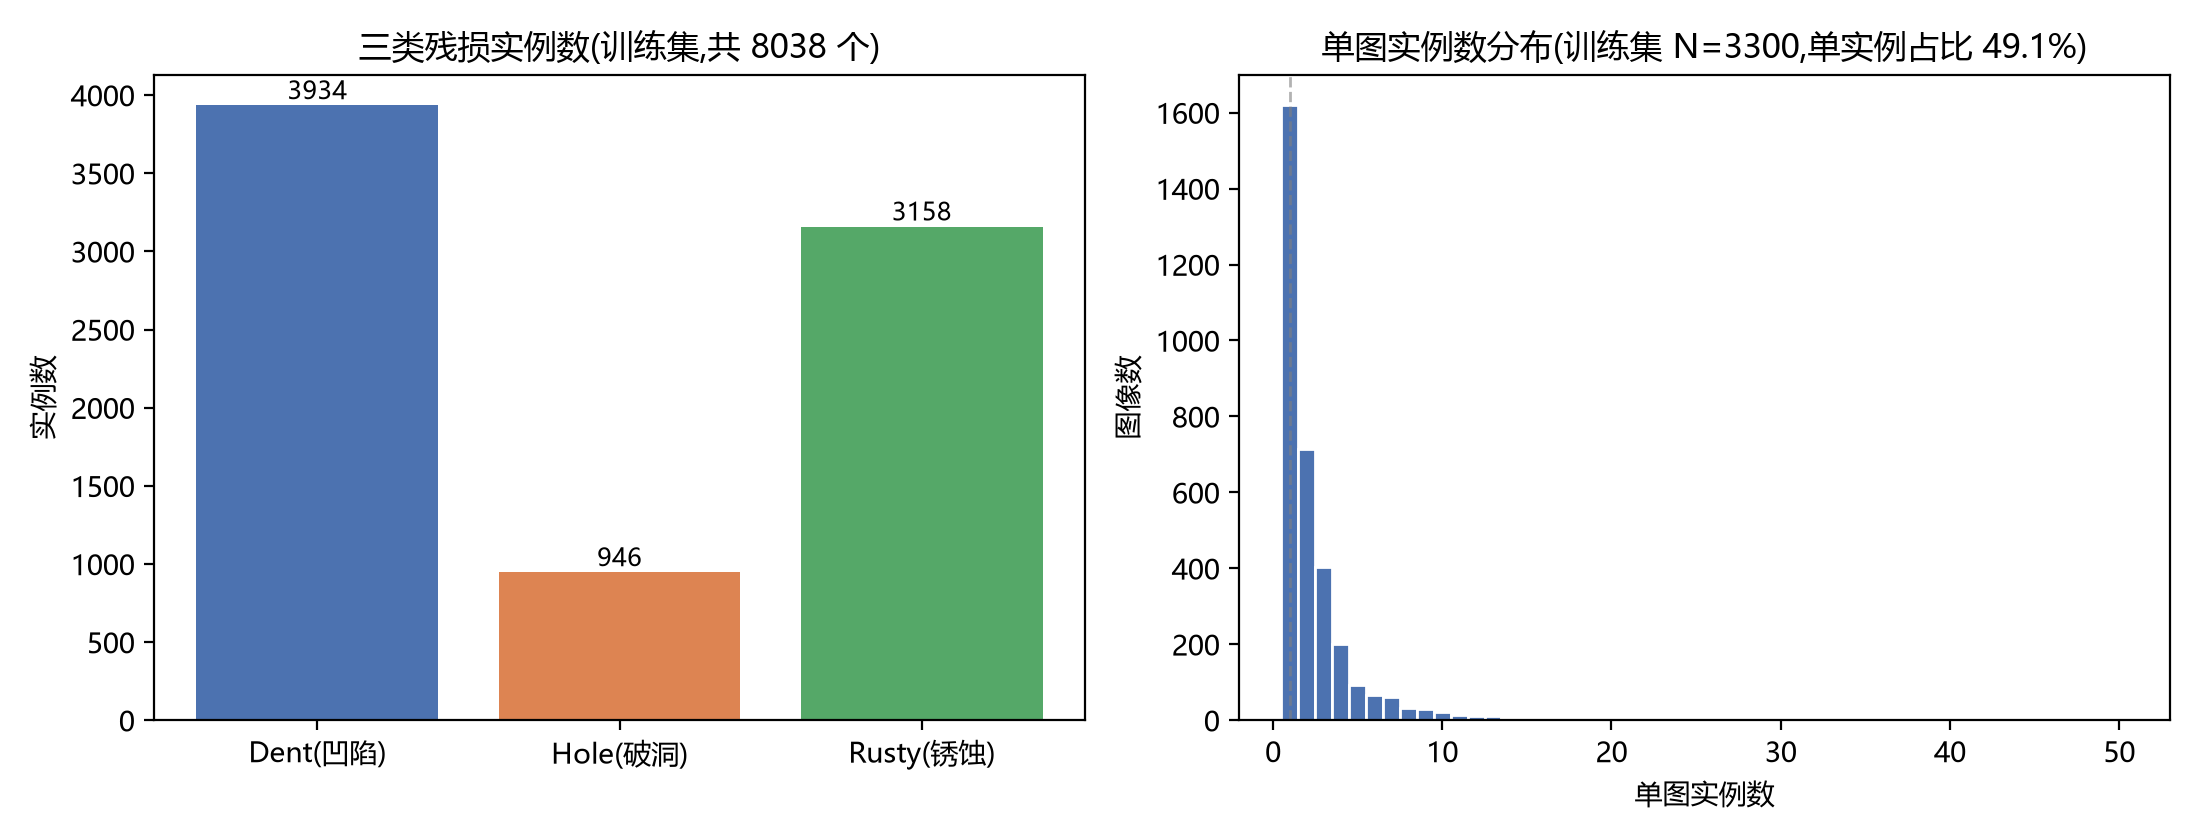
\includegraphics[width=0.95\textwidth]{figures/fig_data_dist.png}
% \caption{数据分布(左:三类残损实例数;右:单图实例数直方图)}
% \label{fig:data-dist}
% \end{figure}
%
% 待新增图 fig:data-scale(取消注释;由 fig_data_scale.py 生成):
% \begin{figure}[h]
% \centering
% 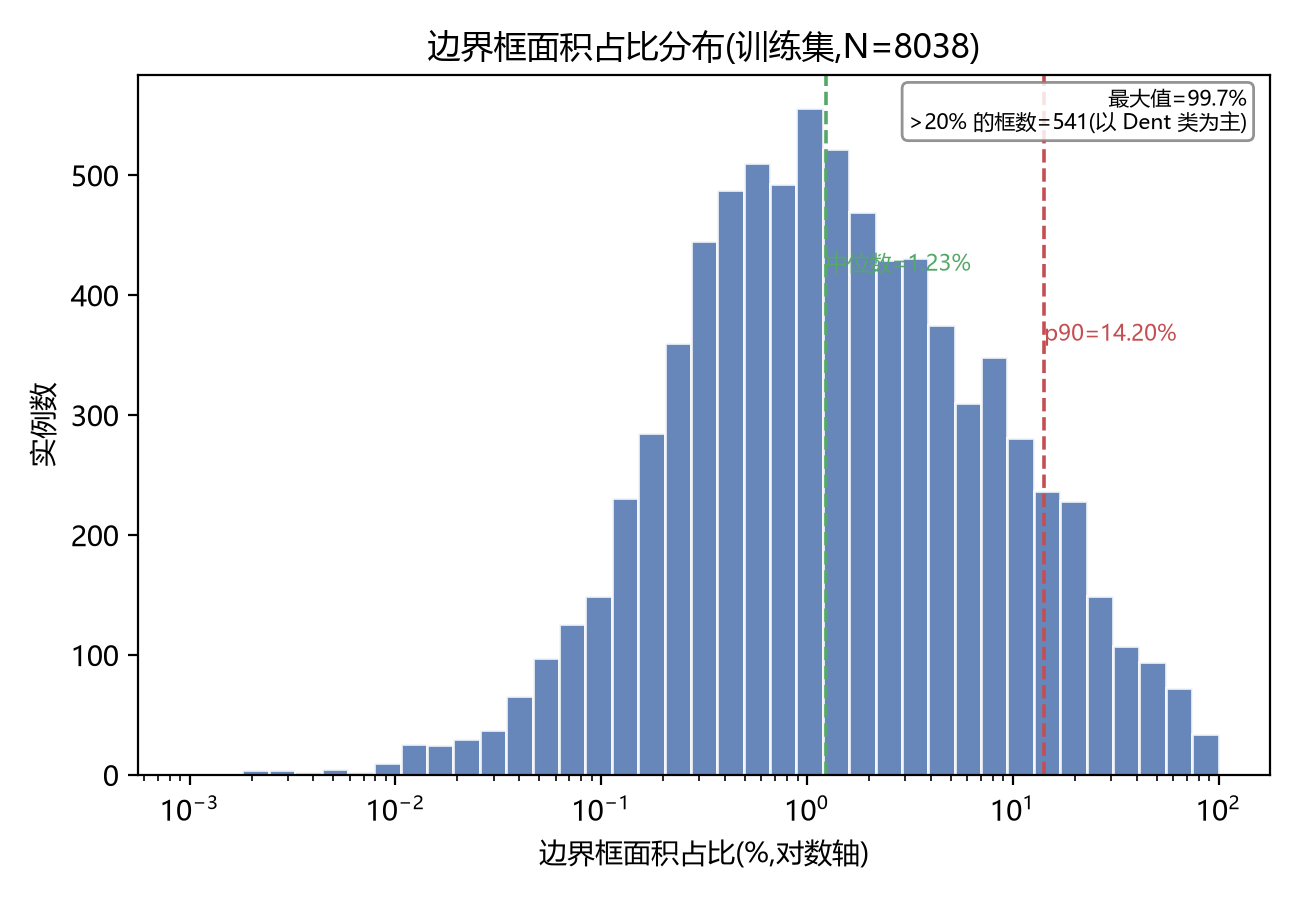
\includegraphics[width=0.6\textwidth]{figures/fig_data_scale.png}
% \caption{边界框面积分布(对数轴)}
% \label{fig:data-scale}
% \end{figure}

\subsection{问题一的分析}

问题一要求判断一张集装箱外表面图像是否存在任何形式的残损,本质上是一个\textbf{二分类问题}:对每张输入图像,输出“存在残损”或“不存在残损”两种判定之一。

从数据看,本题存在两个突出难点。其一,\textbf{训练集缺少负样本}:3300 张训练图像全部含有残损标注,没有任何“无残损”样本,因此无法直接训练有监督的二分类器——若强行训练,分类器只会退化到“恒判有残损”。其二,\textbf{背景复杂、干扰多样}:港口机械、天空、地面等复杂背景,叠加光照变化、反光、阴影、雨水、污渍,使“有无残损”难以仅凭全局外观简单判断;同时残损尺度差异大、类别间(如深凹痕与破洞)外观相似。

针对上述难点,问题一采用“归约为检测”的思路:由于缺少负样本,存在性分类应当等价地转化为残损检测——“是否存在残损”即“图像中能否检测出置信度超过阈值的残损区域”。这一归约绕开了负样本缺失的困境,并使问题一与问题二的检测模型天然统一,构成端到端的统一检测框架。需要说明的是,验证集同样全部含残损标注,评估查准率、误报率与 $AUC$ 时缺少真实负样本;本文以合成负样本(从残损图像中裁取无标注框区域拼合而成)与正样本构成评估集,并将合成负样本划分为调参半与评估半,使阈值选择与最终指标报告相互隔离;负样本合成的有效性在模型假设中说明。最后,用准确率、查准率、召回率、$F_1$ 值与 $AUC$ 等指标对分类效果进行评估。

\subsection{问题二的分析}

问题二要求在检测到残损后,进一步定位残损位置并识别其具体类别,属于\textbf{目标检测与实例分割}任务:检测分支输出残损的边界框(位置)与类别(凹陷/破洞/锈蚀三类),分割分支输出残损的像素级掩码。这是本题的核心与难点所在。

从数据看,问题二面临三方面困难。其一,\textbf{多尺度}:残损尺度差异大,边界框面积从不足 $0.15\%$ 到约 $14\%$ 图像面积不等,大的如大面积锈蚀,小的如细微破洞,要求模型具备较强的多尺度特征提取能力。其二,\textbf{类别不平衡与相似}:破洞类样本远少于凹陷与锈蚀,且深凹痕与破洞外观相似,易混淆。其三,\textbf{单图多实例}:单张图像残损实例数最多达数十个,需可靠的后处理去重。

针对上述困难,问题二采用\textbf{单阶段实例分割网络}(以 YOLOv8-seg 为代表):以卷积神经网络(CNN)主干提取多尺度特征,经特征金字塔融合后,由解耦检测头同时输出边界框、类别与掩码,端到端地完成检测与分割;并通过多尺度特征、类别加权损失与高分辨率输入缓解小目标与类别不平衡问题。最后,用检测指标(均值平均精度)与分割指标(平均交并比、Dice 系数)分别评估定位分类与分割效果。

\subsection{问题三的分析}

问题三要求对问题一、问题二建立的模型从不同维度进行评估,本质是一个\textbf{模型评估问题}:需要建立系统的评估体系,从准确性、鲁棒性、效率、可解释性等维度检验模型,并通过对比实验与灵敏度分析支撑模型选择的合理性。

评估体系从四个维度展开。一是\textbf{准确性}:对问题一的分类模型用准确率、查准率、召回率、$F_1$ 值与 $AUC$ 检验;对问题二的检测与分割模型用均值平均精度(含不同交并比口径与目标尺度)和平均交并比、Dice 系数分别检验。二是\textbf{鲁棒性}:数据集背景复杂、光照多变,通过对验证集施加定量扰动(亮度、对比度、噪声、模糊)模拟真实干扰,考察性能衰减。三是\textbf{效率}:港口场景要求实时性,以推理帧率与参数量评估部署可行性。四是\textbf{可解释性}:用 Grad-CAM 可视化模型关注区域,验证其聚焦残损而非背景。

此外,设计两组支撑性实验:对比实验(检测归约方案与自建小 CNN、传统特征的对比;不同骨干规模模型的对比)与消融实验(类别加权、小目标增强、高分辨率等措施逐一验证),并对置信度阈值、NMS 阈值、top-4 排序方式、输入分辨率等关键超参作灵敏度分析,从而全面、定量地回答“模型好不好、好在哪、稳不稳”。
